\chapter{Background}
\label{chap:background}

This chapter introduces the used packages, including Docker, Docker Swarm, and CRIU (Checkpoint-and-Restore In Userspace).

\section{Docker}
Docker is an open-source container engine, which provides an additional layer of abstraction and automation of operating-system-level virtualization in Linux.  Moreover, Docker has extra image management and layered file system to optimize the performance of container and to reduce disk space. Docker images and Docker containers share the same image layer file if they have the same data. To initialize a container, Docker creates a writable layer that allow the container application to change file system.  

\begin{figure}[h]
\begin{center}
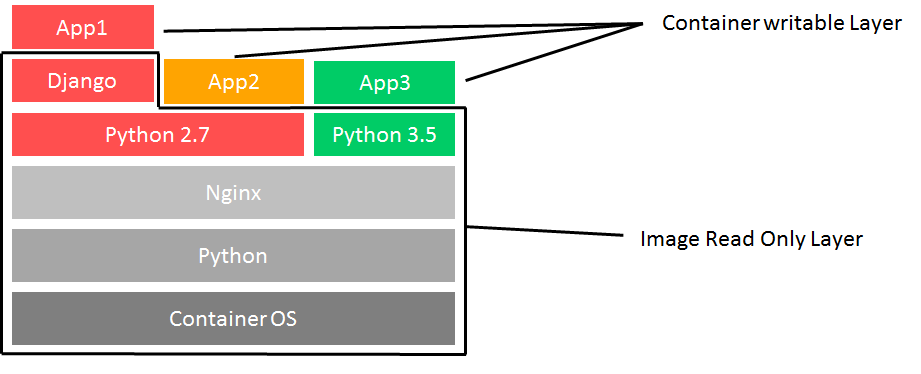
\includegraphics[width=15cm]{figure/layered_file_system.png}
\end{center}
\caption{Docker layered file system}
\label{fig:Docker layered file system}
\end{figure}

\begin{figure}[h]
\begin{center}
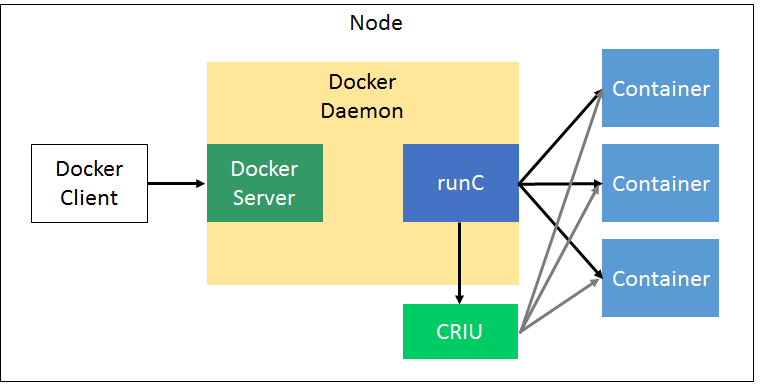
\includegraphics[width=10cm]{figure/single_node.png}
\end{center}
\caption{Single node Docker}
\end{figure}

Docker is a typical client-server architecture, which consists of two parts: Docker client and Docker daemon. Docker client provides the CLI (Command Line Interface) to send/receive requests to/from Docker Daemon.  Also, Docker supports RESTful API \cite{christensen2009using} to communicate with Docker daemon. Docker daemon runs as system service, which serves three  importance functions: 
\begin{itemize}
    \item Receive and handle requests from Docker clients.
    \item Manage containers.
    \item Manage container images.
\end{itemize}
When running, a Docker daemon will receive requests from Docker clients or remote RESTful API. After receiving requests, daemon will pass the requests to a router, which finds the corresponding functions to handle the requests. By default, Docker daemon listens to UNIX socket requests.  To receive remote RESTful APIs or Docker Swarm requests, the daemon listens to the TCP socket.

\subsection{runC}
After version 0.9, Docker used \emph{libcontainer} as its default execution environment, and \emph{runC} \cite{runc} is a repackaging of \emph{libcontainer}, which provides CLI to support the containers management, such as the control of namespace, cgroups, apparmor, network, capabilities, firewall, etc.

\section{Docker Swarm}
Docker Swarm is an orchestration tool for Docker, which gathers several Docker engines together into one virtual Docker engine. Docker Swarm provides standard Docker API, so it can be connected by Dokku, Docker Machine, Docker Compose, Jenkins, DockerUI, Drone, etc. Of course, it also supports Docker client as well.

Docker Swarm has two components: Swarm manager and Swarm node. A Swarm manager is the manager which handles the requests from Docker client and RESTful API and manages multiple Docker nodes'. A Swarm node is an agent which sends heartbeats to the discovery service to ensure the Docker daemons are alive in the cluster.

\begin{figure}[h]
\begin{center}
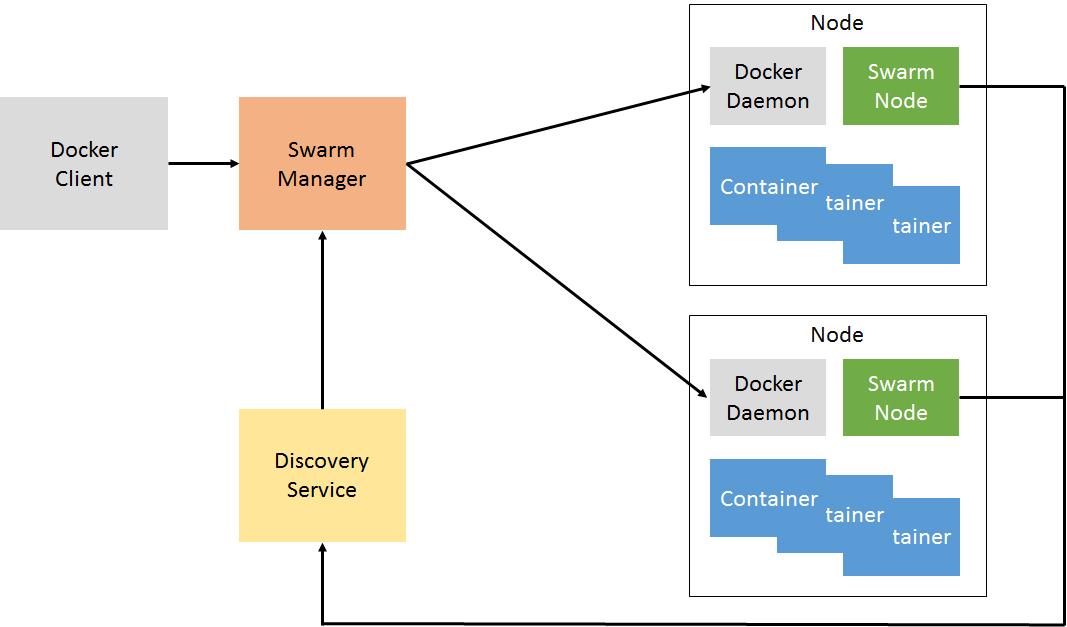
\includegraphics[width=15cm]{figure/swarm_docker.png}
\end{center}
\caption{Docker Swarm architecture}
\end{figure}

\subsection{Discovery services}
Docker Swarm provides multiple Discovery Services in the back-ends, which are used to discover the nodes in the cluster. There are:
\begin{itemize}
    \item Using a distributed key/value store, like Consul, Etcd and Zookeeper.
    \item A static file or list of nodes.
    \item Docker Hub as a hosted discovery service.
\end{itemize}
In addition, it supports any modules that satisfy Discovery API interface.

\subsection{Scheduler}
Docker Swarm scheduler decides which nodes to use when creating and running a container. The scheduling has two steps:
First, the scheduler follows user's filters to decide which nodes can be used.
Second, the scheduler undergoes multiple strategies to select the best node in the cluster.

\subsection{High availability of Swarm Manager}
Swarm Manager responds to the cluster and manages the resources of multiple Docker Daemons which are served by Swarm Nodes. If the Swarm manager dies, a new one will be created to handle with the interruption of service.

The high availability feature allows Docker Swarm has multiple Swarm Manager instances. System manager can create a primary manager and multiple replica instances.
Whenever requests are sent to replica instances, requests will be automatically proxied to the primary manager.
In addition, if the primary manager fails, the other replica instances will lead a new primary manager.

\subsection{High availability of Docker Swarm containers}
Docker Swarm has a rescheduling policy, which can be set when a container is started.  Whenever Swarm nodes fail, Swarm manager will restart all of the containers in that Swarm node to other alive Swarm Nodes.

\section{CRIU}
CRIU \cite{CRIU} (Checkpoint/Restore in Userspace) is a package for checkpointing and restoring of a process.  The checkpointing creates a complete snapshot of a process's state, including  memory contents, file descriptors, and open TCP connections.  CRIU can be used for suspending and resuming processes, or migrating them from one machine to another.

\subsection{Checkpoint}
The checkpoint procedure relies on /proc file system which CRIU takes the information of process.  It needs the pipes parameters, descriptors information, and memory maps. There are 3 steps:
\begin{enumerate}[Step 1.]
	\item Walk through the /proc/\$pid/task directory recursively and collect the process tree.
    \item Collect tasks' resources and dump to the image files.  If the request is pre-dump, CRIU will just collect process tree, and memory pages.  Otherwise, it will collect process tree, memory pages, namespaces, cgroups, share memory, and networks, etc.  While checkpoint request parameter has track-memory, CRIU will compare checkpoint images and memory pages to reduce storage space.
    \item After dumped, CRIU detaches from tasks and they continue to
execute.
\end{enumerate}

\subsection{Restore}
When CRIU restores the process, it will morph itself into the tasks it restore.   There are 4 steps:
\begin{enumerate}[Step 1.]
	\item CRIU reads image files and resolves which processes share with which resources.  Later shared resources are restored by someone process and all the others either inherit one on the 2nd stage (like session) or obtain in some other way.
    \item CRIU calls fork() procedure many times by process tree to create the processes which are needed to be restored.
    \item Restores all resources such as memory mappings, timers, namespaces, cgroups, threads, etc.
    \item Morph CRIU itself into the tasks and continue the process.
\end{enumerate}

\section{Related Work}
The migration of Virtual Machine \cite{clark2005live, liu2013performance} has been researched for a long time.
However, it always has to take a long time because Virtual Machine's resources such as memory, and image spaces are large.

Container migration is a growing researches. Most of researches used checkpoint and restoration to accomplish container migration.
Checkpoint-restoration of Linux applications \cite{laadan2010linux} was a project since 2008. CRIU (Checkpoint/Restore in Userspace) is a project to implement checkpoint/restore functionality for Linux in userspace.
In \cite{yang2015checkpoint}, it used CRIU to migrate Docker container.
\cite{mirkin2008containers} used checkpoint to live migrate OpenVZ container.